\documentclass[a4paper,12pt]{article}

% Paquetes necesarios
\usepackage[utf8]{inputenc}   % Codificación de caracteres
\usepackage[spanish]{babel}   % Idioma español
\usepackage{amsmath, amssymb} % Símbolos matemáticos
\usepackage{graphicx}         % Inclusión de gráficos
\usepackage{cite}             % Gestión de citas
\usepackage{hyperref}         % Enlaces y referencias
\usepackage{geometry}         % Configuración de márgenes
\usepackage{fancyhdr}         % Encabezados y pies de página
\usepackage{titlesec}         % Formato de títulos
\usepackage{booktabs}         % Tablas profesionales
\usepackage{caption}          % Personalización de leyendas
\usepackage{enumitem}         % Personalización de listas
\usepackage{float}

% Configuración de márgenes
\geometry{left=3cm, right=3cm, top=2.5cm, bottom=2.5cm}

% Configuración de encabezados y pies de página
\setlength{\headheight}{14.49998pt}
\pagestyle{fancy}
\fancyhf{}
\fancyhead[L]{Universidad de Granada}
\fancyhead[R]{Escuela Superior Ténica de Ingeniería Informática}
\fancyfoot[L]{Ismael Sallami Moreno}
\fancyfoot[C]{\thepage}
\fancyfoot[R]{\today}

% Formato de títulos
\titleformat{\section}{\large\bfseries}{\thesection.}{0.5em}{}
\titleformat{\subsection}{\normalsize\bfseries}{\thesubsection.}{0.5em}{}

% Datos del documento
\title{\textbf{Práctica 0 de Fundamentos de Ingeniería del Software}}
\author{
    Ismael Sallami Moreno \\
    \texttt{ism350zsallami@correo.ugr.es}
}
\date{
    \vspace{1cm}
    \begin{tabular}{rl}
        \textbf{Asignatura:} & Fundamentos de Ingeniería del Software \\
        \textbf{Tema:} & Uso de la Herramienta Visual Paradigm \\
        \textbf{Fecha:} & \today
    \end{tabular}
}

\begin{document}

% Portada
\maketitle
\begin{center}
    
\includegraphics[width=0.5\textwidth]{images/logo_ugr.png}
\end{center}
\newpage

% Resumen
\begin{abstract}
\noindent
En este documento se adjunta las imagenes de los diagramas de clases, casos de uso y secuencia realizados en la herramienta Visual Paradigm. Además, se incluye una breve descripción de cada uno de los diagramas y se explica cómo se han generado. Como todos se han realizado de la misma forma la explicación será la misma para todos los diagramas o similar.\\
\end{abstract}
\bigskip

% Palabras clave
\noindent
% \textbf{Palabras clave:} plantilla, LaTeX, trabajos académicos, tecnología
% \newpage

% Tabla de contenidos
\tableofcontents
\newpage

% Introducción
\section{Diagrama de casos de uso}
En este caso se nos pedía realizar un diagrama de casos de uso, el cual nos queda de la siguiente forma:

\begin{figure}[H]
    \centering
    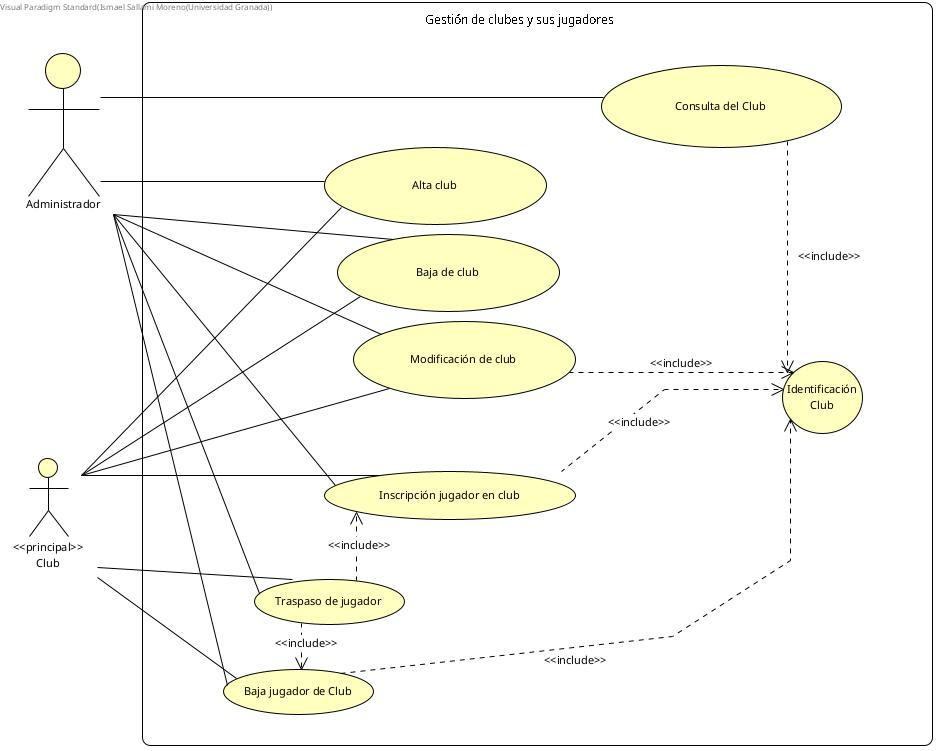
\includegraphics[width=1\textwidth]{Diagrama_de_casos_de_uso.jpg}
    \caption{Diagrama de casos de uso}
    \label{fig:casos_de_uso}
\end{figure}

\newpage
\section{Modelo Conceptual}
En este caso se nos pedía realizar un diagrama de clases, el cual nos queda de la siguiente forma:

\begin{figure}[H]
    \centering
    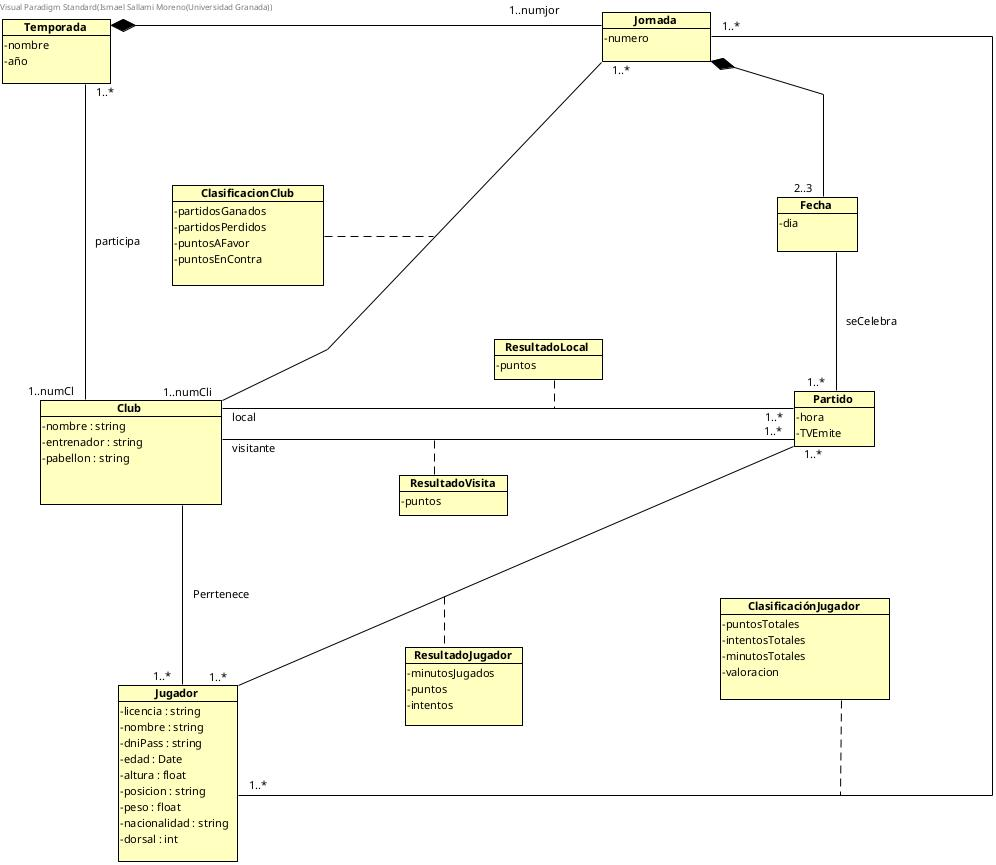
\includegraphics[width=1\textwidth]{Modelo_Conceptual.jpg}
    \caption{Modelo Conceptual}
    \label{fig:modelo_conceptual}
\end{figure}

\newpage
\section{Diagrama de secuencia del sistema}

En este caso se nos pedía realizar un diagrama de secuencia, el cual nos queda de la siguiente forma:

\begin{figure}[H]
    \centering
    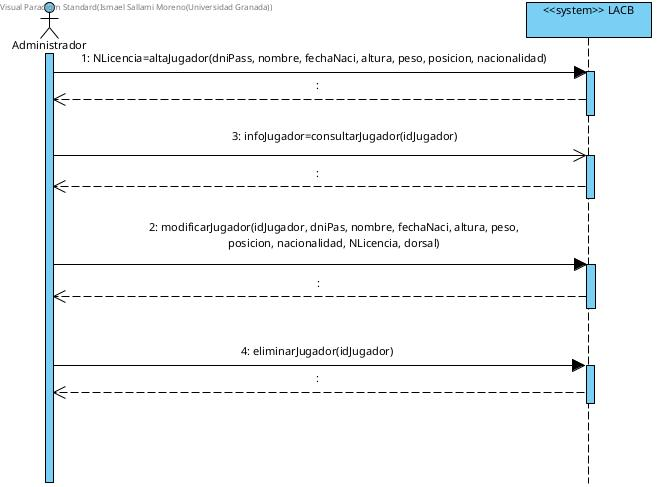
\includegraphics[width=1\textwidth]{Secuencia_Sistema.jpg}
    \caption{Diagrama de secuencia del sistema}
    \label{fig:secuencia_sistema}
\end{figure}




% Referencias
\newpage
\begin{thebibliography}{99}
\bibitem{Referencia1}
Autor(es), \emph{Título del artículo}, Nombre de la Revista, volumen(número), páginas, año.

\bibitem{Referencia2}
Autor(es), \emph{Título del libro}, Editorial, año.

\bibitem{Referencia3}
Autor(es), \emph{Título del documento}, Nombre de la Conferencia, páginas, año.
\end{thebibliography}

\end{document}
